\documentclass[12pt]{scrartcl}

\usepackage[all,blueheadings,150]{HSMW-Logo}
\usepackage[utf8]{inputenc} 			% wichtig für Umlaute
\usepackage[onehalfspacing]{setspace} % Zeilenabstand 1,5 Fach
\usepackage[ngerman]{babel}
\setlength{\parindent}{0pt} % Neue Absätze nicht einrücken
\usepackage{hyperref}
\setcounter{tocdepth}{1}	% Nur die erste Ebene im Inhaltsverzeichnis anzeigen.
\usepackage{rotating}
\usepackage{pdflscape}

%Anhang


\begin{document}
	
	
	%\titlehead{Kopf der Titelei}
	\subject{Verteilte Systeme}
	\title{Programmier-Beleg REST}
	\subtitle{Eine zentrale Projektverwaltung für Studenten und Professoren}
	\author{Felix Haller (fhaller1) \and Konstantin Lorenz (klorenz1)}
	\date{07.10.2015}
	\publishers{Prüfer: Prof. Dr.-Ing. Andreas Ittner}
	%\extratitle{\centering Schmutztitel \\ goLaTeX (C) 2009 \\ ISBN 978-3865412911}
	%\uppertitleback{Obiger Titelrückentitel}
	%\lowertitleback{Für dieses Beispiel wird keine Haftung übernommen.}
	%\dedication{Dieses Beispiel widme ich\\allen LaTeX Usern}
	\maketitle
	\thispagestyle{empty} 
	\newpage
	\tableofcontents
	\thispagestyle{empty}
	\newpage	
	\setcounter{page}{1} 
	
	
	
	\section{Aufgabenstellung}
		Nachfolgend weitestgehend übernommen aus offizieller Aufgabenstellung:
		Es soll im Rahmen einer Belegarbeit ein eigener, lauffähiger RESTful Webservice mit einem frei wählbaren Thema entwickelt
		werden. Zum Nachweis der Funktionsfähigkeit ist ein Testclient notwendig, der ein Testszenario nachvollziehbar durchspielt und damit alle Funktionen des Service prüft. In der abzugebenden technischen Dokumentation soll alles enthalten sein, was zum Verständnis des Services, also seiner Funktion und dem technischen Hintergrund, notwendig ist.
		
	\section{Motivation}
		Zur Zeit existiert keine zentrale Anlaufstelle, wenn es um die Bekanntmachung von und die Suche nach Projekten geht. Das Ziel des Webservice ist eine bessere Vernetzung der Hochschulmitglieder während der Planung und Durchführung von Projekten. Einerseits soll eine Möglichkeit für Professoren gegeben werden geplante Forschungsarbeiten, für die noch Unterstützer gesucht werden, vorzustellen. Andererseits soll Studenten die Möglichkeit geboten werden bei Interesse an einem Thema - beispielsweise einer bestimmten Programmiersprache - eine Anlaufstelle zur praktischen Umsetzung zu finden. Außerdem erleichtert es u.U. das Finden eines Themas für praktische Belegarbeiten (z.B. Java2, Verteilte Systeme, SWT, ...)
	\section{Installations- und Startanleitung}
		Das Projekt wird mittels des Build Systems \emph{gradle} entwickelt. Es hilft bei den regelmäßig auszuführenden Arbeiten, wie dem Kompilieren von Klassen, dem Testen der Anwendung und der Erstellung der Javadoc Dokumentation. Innerhalb der gradle Konfigurationsdateien wurden Abhängigkeiten so definiert, dass beim Bau des Hauptprojektes alle Unterprojekte gleich mit gebaut und getestet werden. Außerdem werden alle benötigten Abhängigkeiten beim erstmaligen Kompilieren der Quellen heruntergeladen. Somit ist keine manuelle Installation von externen Abhängigkeiten notwendig. Um zuvor gebaute und temporäre Dateien vor dem Kompilieren zu löschen empfiehlt es sich den \emph{clean} Auftrag vorher auszuführen.
				
		Zum Erstellen und Testen des gesamten Projektes verwendet man also den folgenden Befehl:
		\begin{verbatim}
			$ gradle clean build
		\end{verbatim}
		
		Zum Starten des REST-Service verwendet man den entsprechenden Auftrag innerhalb des \emph{rest} Projektes:
		\begin{verbatim}
			$ gradle rest:jettyRun
		\end{verbatim}
		
		Danach ist der Service unter der Adresse http://localhost:8080 erreichbar und gemäß den in Abschnitt \ref{sec:restschnittstellen} beschriebenen Methodenaufrufen verwendbar.
		
		Die Verwendung des mitgelieferten Clients wird in Abschnitt \ref{sec:client} ausführlich erklärt.
	\section{REST Ressourcen im Überblick}
		%Konstantin
		Wie in der Abbildung \ref{fig:rest} zu sehen


	\section{REST-Schnittstellen} \label{sec:restschnittstellen}
\subsection{Projekte}
	Projekte sind das zentrale Element, die jeder anlegen kann und an denen jeder Interessierte teilhaben kann. Ob es nun darum geht bei einem Projekt immer auf dem aktuellen Stand zu bleiben oder aktiv mitzuarbeiten.
	\begin{itemize}
			\item \emph{/projects}, ist eine Ressource, die ein Projekt darstellt. 
			\begin{itemize}
				\item GET, listet alle in der Datenbank verfügbaren Projekte auf, die den Status \emph{published} oder \emph{closed} besitzen
				\begin{itemize}
					\item Query Parameter: \emph{title, tag, creator} sind alle optional und dienen der Einschränkung der Projektausgabe. Dabei kann eine Filterung über den Projekt-Title, die zugehören Tags sowie über den Ersteller vorgenommen werden. Es werden nur Projekte angezeigt, die den Status \emph{published} oder \emph{closed} besitzen.
					\item Rückgabewerte: Es wird eine Liste von Projekten, die der Filterung entsprechen, zurückgegeben. Falls keine Übereinstimmung bei der Filterung erfolgt, wird ein Statuscode 204 gesendet. 
				\end{itemize}
				\item POST, Es wird ein neues Projekt erzeugt und in die Datenbank eingetragen.
				\begin{itemize}
					\item Form Parameter:
					\begin{itemize}
						\item  \emph{title}, Titel des Projektes als String
						\item  \emph{username}, Benutzername des Erstellers. Der Ersteller muss als User in der Datenbank vorhanden sein.
						\item  \emph{description}, Beschreibung des Projektes als String
						\item  \emph{members}, Mitarbeiter mit ihren Rollen mit folgender Syntax: username1,Rolle;username2,Rolle; Die Mitarbeiter müssen als User in der Datenbank vorhanden sein. Die Rollen können frei gewählt werden.
						\item  \emph{tagname (optional)}, Tag-Name eines vorhandenen Tags
						\item \emph{postsURL}, URL eines RSS-Feeds 
					\end{itemize}
					\item Rückgabewerte: Es wird das erstellte Projekt-Objekt zurückgegeben. Der zugehörige Statuscode ist 200. Ist ein nicht optionaler Parameter leer oder wird gegen die Syntax verstoßen, ist ein Statuscode 406 zu erwarten.  
				\end{itemize}
			\end{itemize}
			\item \emph{/projects/\{id\}} Hier kann die \emph{id} des Projektes angegeben werden. Alle Methoden werden zur Manipulation des Projektes mit dieser \emph{id} verwendet.
			\begin{itemize}
				\item GET, ruft das Projekt ab und stellt es dar. 
				\begin{itemize}
					\item Path Parameter: \emph{id}, Nummer des Projekts
					\item Rückgabewerte: Falls ein Projekt mit dieser \emph{id} nicht vorhanden ist, wird ein Statuscode 404 erzeugt. Ansonsten wird das Projekt mit dem Statuscode 200 zurückgegeben.
				\end{itemize}
				\item PUT, das Projekt kann mit dieser Methode verändert werden. Alle Parameter sind optional. Erfolgt keine Wertzuweisung bei den Parametern, gibt es auch keine Änderung. Die Parameter liegen in gleicher Weise vor, wie bei der POST-Methode von der \emph{/projects} Ressource.
				\item DELETE, Das Projekt-Objekt mit der zugehörigen \emph{id} wird gelöscht.
				\begin{itemize}
					\item Rückgabewerte: Es wird das gelöschte Projekt-Objekt mit einem Statuscode 200 zurückgegeben. Ist diese \emph{id} nicht vorhanden, wird ein Statuscode 404 gesendet.
				\end{itemize}	
			\end{itemize}
	\end{itemize}
\subsection{Kommentare}
	Die Kommentare dient den Benutzern des \emph{Project-Hub} als Rückkanal für die Betreiber des Projektes. Damit ist es möglich Verbesserungsvorschläge, Anregungen, Wünsche aber auch Kritik anzubringen und somit eine höhere Qualität und Benutzerfreundlichkeit von Projekten zu erreichen.  
	\begin{itemize}
		\item \emph {projects/\{id\}/comments}, ist eine Ressource, die einen Kommentar darstellt.
		\begin{itemize}
			\item GET, listet alle in der Datenbank verfügbaren Kommentare auf, die zu der \emph{id} des Projektes gehören und  den Status \emph{published} oder \emph{closed} besitzen
			\begin{itemize}
				\item Rückgabewerte: Es wird eine Liste von Kommentaren, die zu der Projekt-\emph{id} des Projektes gehören, ausgegeben. Der Statuscode ist bei erfolgreicher Rückgabe 200. Falls keine Kommentare vorhanden sind, wird ein Statuscode 204 zurückgegeben. Es werden nur Kommentare angezeigt, die den Status \emph{published} oder \emph{closed} besitzen.
			\end{itemize}
					\item POST, Es wird ein neuer Kommentar erzeugt und in die Datenbank eingetragen.
					\begin{itemize}
						\item Form Parameter:
						\begin{itemize}
							\item  \emph{title}, Titel des Kommentars als String
							\item  \emph{creator}, Benutzername des Erstellers. Der Ersteller muss als User in der Datenbank vorhanden sein.
							\item  \emph{content}, Inhalt des Kommentars als String
							\item  \emph{status}, Hier kann der Status des Kommentars angegeben werden. Es sind folgende Wert möglich: \emph{new, published, closed}.
						\end{itemize}
						\item Rückgabewerte: Es wird das erstellte Kommentar-Objekt zurückgegeben. Der zugehörige Statuscode ist 200. Ist ein Parameter leer oder wird gegen die Syntax verstoßen, ist ein Statuscode 406 zu erwarten.  
					\end{itemize}
		\end{itemize}
			\item \emph{projects/\{id\}/comments/\{id\}} Hier kann die \emph{id} des Kommentars angegeben werden. Alle Methoden werden zur Manipulation des Kommentars mit dieser \emph{id} verwendet.
			\begin{itemize}
					\item GET, ruft den Kommentar ab und stellt ihn dar. 
					\begin{itemize}
						\item Rückgabewerte: Falls ein Kommentar mit dieser \emph{id} nicht vorhanden ist, wird ein Statuscode 404 erzeugt. Ansonsten wird der Kommentar mit dem Statuscode 200 zurückgegeben.
					\end{itemize}
					\item PUT, der Kommentar kann mit dieser Methode verändert werden. Alle Parameter sind optional. Erfolgt keine Wertzuweisung bei den Parametern, gibt es auch keine Änderung. Die Parameter liegen in gleicher Weise vor, wie bei der POST-Methode von der \emph{projects/\{id\}/comments} Ressource.
					\item DELETE, Das Kommentar-Objekt mit der zugehörigen \emph{id} wird gelöscht.
					\begin{itemize}
						\item Rückgabewerte: Es wird das gelöschte Kommentar-Objekt mit einem Statuscode 200 zurückgegeben.
					\end{itemize}
			\end{itemize}
	\end{itemize}
\subsection{Posts}
Meistens werden Projekte auf anderen Plattformen entwickelt z.B. Web-Management-Software. Es entsteht unerwünschte Redundanz, deshalb war das Ziel RSS-Feeds mit aktuellen Informationen auf der Projektseite anzubieten, um einen umfangreichen Überblick zu gewährleisten und Redundanz zu vermeiden bzw. zu minimieren.    
	\begin{itemize}
		\item \emph{/projects/\{id\}/posts}, ist ein RSS-Feed einer in der Datenbank hinterlegten URL. Ein RSS-Feed besteht aus mehreren Posts mit einer jeweiligen \emph{id}.
		\begin{itemize}
			\item GET, listet alle Posts eines RSS-Feeds auf, die zu einem Projekt gehören.
			\begin{itemize}
				\item Rückgabewerte: Es werden mehrere Posts eines Feeds des dazugehörigen Projektes ausgegeben. Diese wird bei der Projekterstellung als \emph{postsURL} Parameter verlangt. Ist kein RSS-Feed-URL vorhanden, wird ein Statuscode 204 ausgegeben. Ansonsten ist bei erfolgreicher Ausführung ein Statuscode 200 zu erwarten.
			\end{itemize}
		\end{itemize}
		\item \emph{/projects/\{id\}/posts\{id\}}
		\begin{itemize}
			\item GET, listet ein Post eines RSS-Feeds auf.
			\begin{itemize}
				\item Rückgabewerte: Es wird ein Post eines RSS-Feeds angezeigt. Der dazugehörige Statuscode ist 200. Kann eine \emph{id} keinem Post zugeordnet werden, wird der Statuscode 404 ausgegeben.  
			\end{itemize}
		\end{itemize} 	
	\end{itemize}
\subsection{Schlagworte}
Schlagworte werden hier Synonym zu Tags verwendet.
Tags dienen der näheren Beschreibung und Klassifizierung eines Projektes. Es ist eine uneingeschränkte Zuordnung solcher Schlagworte möglich. Werden Tags konsequent an Projekte vergeben, kann z.B. eine Suche zu einen Schlagwort ausgeführt werden. 
\begin{itemize}
	\item \emph{/tags}, ist die Ressource, die die Tags repräsentiert.
	\begin{itemize}
		\item GET, listet alle vorhanden Tags in einer Liste mit Beschreibung aus.
		\begin{itemize}
			\item Rückgabewerte: Gibt alle Tags, die in der Datenbank vorhanden sind, aus. Bei Erfolg wird der Statuscode 200 erzeugt. Sind keine Tags vorhanden wird ein Statuscode 204 gesendet. 
		\end{itemize}
		\item POST, Es wird ein neues Tag-Objekt erstellt und in der Datenbank abgelegt. Es können keine Tags doppelt angelegt werden.
		\begin{itemize}
			\item Form Parameter: Die Parameter \emph{tagName, description} sind alles Pflichtfelder. \emph{tagName} darf keine Sonderzeichen oder Zahlen enthalten. Die Beschreibung ist frei wählbar. 
		\end{itemize} 
	\end{itemize}
	\item \emph{/tags/\{tagName\}} Einzelner Tag mit einem \emph{tagName} als Name des Tag-Objektes.
	\begin{itemize}
		\item GET, gibt das einzelne Tag-Objekt zurück.
		\begin{itemize}
			\item Rückgabewerte: Bei erfolgreicher Anzeige des Objektes wird ein Statuscode 200 generiert. Ist das Objekt mit diesem \emph{tagName} nicht vorhanden wird ein Statuscode 404 ausgegeben.
		\end{itemize}
		\item PUT, diese Methode dient zum Updaten des Tag. Allerdings ist nur eine Änderung der Beschreibung möglich. Möchte man den Namen ändern, muss ein neue Tag-Objekt erstellt werden.
		\begin{itemize}
			\item Form Parameter: Der einzige Parameter der geändert werden kann:\emph{description}. Wird kein Parameter angegeben oder ist der Parameter leer, erfolgt keine Änderung. 
			\item Rückgabewerte: Wird ein Update erfolgreich ausgeführt, wird der Statuscode 200 generiert und das aktuelle Tag-Objekt angezeigt. Falls das Tag-Objekt mit diesem \emph{tagName} nicht vorhanden ist, wird ein Statuscode 404 ausgegeben.  
		\end{itemize} 
		\item DELETE, löscht einen Tag. Der Tag kann nur gelöscht werden, wenn dieser in keinem Projekt-Objekt mehr verwendet wird.
		\begin{itemize}
			\item Rückgabewerte: Es wird ein Statuscode 200 generiert, wenn das Objekt erfolgreich gelöscht werden konnte. Falls das Objekt mit diesem \emph{tagName} nicht vorhanden ist, kommt es zum Statuscode 404. Wird der Tag noch von einem Projekt verwendet, wird der Statuscode 409 (Conflict) generiert.
		\end{itemize}
	\end{itemize} 	
\end{itemize}
\subsection{Benutzer}
Der Bentzer, in der Ressource als \emph{user} bezeichnet, dient zur eindeutigen Identifikation von Publikationen und soll bei Umsetzung des Projektes aus einer bestehenden Datenbank importiert werden, weshalb davon abgesehen wird Methoden zur Erstellung und Bearbeitung zu implementieren.
\begin{itemize}
	\item \emph{/users}, steht für die \emph{Users} Ressource. 
	\begin{itemize}
		\item GET, Es werden alle Benutzer, die in der Datenbank verfügbar sind, abgerufen und als Liste ausgegeben.
		\begin{itemize}
			\item Rückgabewerte: Bei Erfolg wird eine Benutzerliste mit dem Statuscode 200 übertragen. Ist die Datenbank leer wird der Statuscode 204 erzeugt.
		\end{itemize} 
	\end{itemize}
	\item \emph{ /users/\{id\}}, dient als Ressource für einen einzelnen Nutzer. Über die \emph{id} kann ein Nutzer eindeutig identifiziert werden. 
	\begin{itemize}
		\item GET, Methode zum Abrufen des Nutzers
		\begin{itemize}
			\item Rückgabewerte:Bei erfolgreicher Übertragung wird ein Statuscode 200 ausgegeben. Falls die \emph{id} nicht vorhanden ist, kommt es zu einem Statuscode 404.
		\end{itemize} 
	\end{itemize}
\end{itemize}

\subsection{Neuigkeiten}
Diese Ressource dient dazu die Benutzer über aktuelle Projekte zu informieren. In der Zukunft soll diese Funktion auch aktuelle RSS-Posts ausgeben.
\begin{itemize}
	\item\emph{/recent}, dient als Referenzpunkt für weitere Entwicklungen in der Zukunft.
	\item\emph{/recent/projects}, steht für die neusten Projekte, die den Status \emph{published} besitzen.
	\begin{itemize}
		\item GET, Die Methode ruft die neusten 10 Projekte ab und gibt diese als Liste nach Datum sortiert aus.
		\begin{itemize}
			\item Rückgabewerte: Bei erfolgreicher Rückgabe der Projektliste wird ein Statuscode 200 erzeugt. Anderenfalls wird ein Statuscode 204 z.B. bei einer leeren Liste generiert.
		\end{itemize}
	\end{itemize} 
\end{itemize}
	\section{Datenmodell und Persistierung}
	Zur Persistierung der Daten wird ein relationales Datenbanksystem namens SQLite eingesetzt. Die Datenbank ließ sich ohne weitere Serversoftware einbinden. Zur Anbindung wird der JDBC-Treiber benutzt. Die gesamte Datenbank befindet sich in einer einzigen Datei, der db.sqlite. Diese kann mit der beigefügten createDB.sh neu gebaut werden. In der Datei dbscript.sql befindet sich das dazugehörige SQL-Script mit vielen Beispieldatensätzen. Im produktiven Einsatz ist eine SQLite nicht zweckmäßig und kann durch eine gebräuchlichere Datenbank z.B. MySQL ersetzt werden.  
	
	In der Abbildung\ref{fig:db} ist das Datenbankschema dargestellt. 
	\section{Client}
	\label{sec:client}
		\subsection{Bedienung}
		
			Der Client ist auf der Kommandozeile ausführbar. Gestartet wird er indem man ihn zuerst mit Hilfe von \emph{gradle} baut. Sollte man das gesamte Projekt gebaut haben wird er als Abhängigkeit bereits erstellt.
			\begin{verbatim}
				$ gradle build client
			\end{verbatim}
			
			Danach findet man im Verzeichnis \emph{client/build/distributions} eine \emph{client.tar}, in welcher sich der lauffähige Client befindet. Man muss sie zuerst entpacken und danach den client starten.
			
			\begin{verbatim}
				$ cd client/build/distributions
				$ tar xf client.tar
				$ cd client
				$ bin/client
			\end{verbatim}
			
			Für eine JAR Datei mit allen Abhängigkeiten wurde von uns eine Task \emph{createRunnable} im client Projekt erstellt. Mithilfe von
			\begin{verbatim}
				$ gradle client:createRunnable
				$ java -jar client/build/libs/client-all.jar
			\end{verbatim}
			
			kann diese erzeugt und anschließend gestartet werden.
		\subsection{Methoden des Clients}
		
			Für die einzelnen Aufgaben wurden jeweils Methoden erstellt, die eine Instanz der Apache \emph{HttpClient} Klasse bedienen. Sie senden eine GET/POST/PUT/DELETE Anfrage zum REST-Service und empfangen das Ergebnis. Das anschließende Unmarschalling der empfangenen XML Bäume in die entsprechenden Java-Objekte übernehmen spezielle Methoden für die einzelnen Objekt-Typen.
			
			Für die formatierte Ausgabe der XML-Antworten wurde außerdem eine Klassen-Methode \emph{prettyPrintXml} geschrieben.
		
		
		\subsection{Testszenarien}
			
			Er testet die Funktionalität des REST-Service und gibt die Rückgabe (XML) formatiert aus. Nach jedem Szenario unterbricht er seinen Lauf, um dem Bediener die Möglichkeit zu geben den Ablauf der Abrufe nachzuvollziehen und die Ausgabe zu betrachten. Die Ausführung kann durch das Drücken der ''ENTER'' Taste fortgesetzt werden. Der Client gibt aus, was er gerade macht und was darauf hin passiert. Während des Durchlaufs werden zudem die zurückgelieferten Statuscodes ausgegeben.
			
			Der Client testet folgende Anwendungsszenarien:
			\begin{itemize}
				\item Anzeigen eines bereits vorhandenen Demo - Projektes
				\begin{itemize}
					\item Erwartetes Ergebnis: erfolgreich (Statuscode: 200)
				\end{itemize}
				\item Anzeigen der Kommentare zu einem Projekt
				\begin{itemize}
					\item Erwartetes Ergebnis: erfolgreich (Statuscode: 200)
					\item Es wird der Inhalt des ersten Kommentar ausgegeben
				\end{itemize}
				\item Versuch des Abrufs eines nicht vorhandenen Projektes (falsche ID)
				\begin{itemize}
					\item Erwartetes Ergebnis: Fehler (Statuscode: 404)
				\end{itemize}
				\item Erstellen eines neuen Projektes
				\begin{itemize}
					\item Erwartetes Ergebnis: erfolgreich (Statuscode: 201)
					\item Die ID des angelegten Projektes wird am Ende ausgegeben
				\end{itemize}
				\item Suchen nach Projektnamen
				\begin{itemize}
					\item Erwartetes Ergebnis: erfolgreich (Statuscode: 200)
					\item Anzahl der gefundenen Projekte wird ausgegeben
				\end{itemize}
				\item Modifizieren eines Projektes (zwei Abfragen)
				\begin{itemize}
					\item Tippfehler in Beschreibung wird korrigiert
					\item Tag wird zum Projekt hinzugefügt
					\item Erwartetes Ergebnis: erfolgreich (Statuscode: 200) (beide Male)
				\end{itemize}
				\item Das Filtern von Projekten nach Tags
				\begin{itemize}
					\item Erwartetes Ergebnis: erfolgreich (Statuscode: 200)
					\item Anzahl der mit Tag markierten Projekte wird ausgegeben
				\end{itemize}
				\item Erstellen eines Kommentars zu einem Projekt
				\begin{itemize}
					\item Erwartetes Ergebnis: erfolgreich (Statuscode: 201)
					\item Kommentar-ID wird am Ende ausgegeben
				\end{itemize}
				\item Anzeigen der RSS-Posts zu einem Projekt
				\begin{itemize}
					\item Erwartetes Ergebnis: erfolgreich (Statuscode: 200)
					\item (Abhängig von der Erreichbarkeit des fremden Service. Im Beispiel Projekt handelt es sich um github.com)
					\item Der Inhalt des jüngsten Posts wird angezeigt
				\end{itemize}
				\item Anzeigen der letzten angelegten Projekte
				\begin{itemize}
					\item Erwartetes Ergebnis: erfolgreich (Statuscode: 200)
					\item letzten (max. 10) angelegten Projekte werden absteigend sortiert angezeigt
					\item Die ID des neusten Projektes wird angezeigt
				\end{itemize}
				\item Das Löschen eines Projektes
				\begin{itemize}
					\item Erwartetes Ergebnis: erfolgreich (Statuscode: 200)
					\item Projekt wird in Datenbank als gelöscht markiert
					\item Letzter Zustand des gelöschten Projektes wird ausgegeben
				\end{itemize}
				\item gelöschtes Projekt erneut anzeigen
				\begin{itemize}
					\item Erwartetes Ergebnis: Fehler (Statuscode: 404)
				\end{itemize}
			\end{itemize}
		
	\section{Zusammenfassung}
	Mit diesem Projekt ist es gelungen eine Plattform zu schaffen, die für das Bekanntmachen von Projekten geeignet ist. Es erleichtert den Professoren für neue Projekte zu werben und Mitglieder zu gewinnen, die sich an Projekten beteiligen wollen. Durch Zuordnung von Tags zu den Projekten kann nach individuellen Gesichtspunkten eine Suche zu einem Thema durchgeführt werden. Für Studierende ist es einfacher ein Thema für z.B. eine Belegarbeit zu finden. Durch individuelle Kommentarfunktionen und RSS-Feed Unterstützung ist eine hohe Vernetzung gegeben, die es ermöglicht Projekte zu diskutieren. Die Neuigkeitenfunktion ermöglicht es Studenten und Professoren immer auf dem aktuellen Stand zu halten und Informationen über neue Projekte zu bekannt zu machen. 
	\section{Fazit (Entwurf)}
		\begin{itemize}
			\item viel gelernt
			\item Zeit für Doku unterschätzt
			\item wollten RSS Service (war Bonus) noch integrieren, dadurch zu wenig Zeit für Doku
			\item Arbeiten im Team am Anfang schwierig (Aufwand durch Merge Konflikte und unbekannte Workflows sowie unterschiedliche Programmierstile)
		\end{itemize}
		
	\section{Arbeitsverteilung}
		
		Die Entwicklung erfolgte in enger Zusammenarbeit beider beteiligten. Ganz am Anfang startete Felix Haller mit der Entwicklung eines lauffähigen REST Service mit Demo-Antworten auf REST-Anfragen. Währenddessen erstellte Konstantin Lorenz die zuvor ausgearbeitete Datenbank und ein Skript um diese automatisiert erstellen zu können. Als diese beiden Sachen lauffähig waren, wurde das erste mal getauscht um auch die anderen Bereiche kennen zu lernen. Konstantin Lorenz übernahm die Weiterentwicklung des REST Service um die fehlenden Ressourcen sowie Methoden und Felix Haller programmierte die Schnittstelle zur nun vorhandenen Datenbank so wie die Kapsel-Klassen für alle Objekte.
		Nachdem der Kern-Service lief widmete sich Felix Haller der Schnittstelle zu den RSS Posts. Das beinhaltet den Backend-Service für die zuvor von Konstantin Lorenz vorbereiteten REST Ressource (/projects/{id}/posts). Herr Lorenz begann mit dem Beheben von im Laufe der Tests aufgefallenen Fehlern und dem dazugehörigen Anpassen der Services und der Datenbank.
		
		Nachfolgend eine genauere Aufschlüsselung aller weiteren Teile der Entwicklung und der jeweiligen Arbeitsverteilung:
	 
		
		\subsection{Design des REST Service und gradle Skripte}
			Gemeinsame Arbeit.
		\subsection{Entwicklung REST Service}
			Grundlegender REST Service von Felix Haller erstellt mit einigen Methoden der /projects Ressource. Später weiterentwickelt (/recent..., /user...) durch Konstantin Lorenz. Fehlerbeseitigung in gemeinsamer Arbeit. 
		\subsection{Design der Datenbank}
			Gemeinsame Arbeit.
		\subsection{Erstellung Datenbank}
			Größtenteils durch Konstantin Lorenz parallel zur Erstellung des Grundgerüsts des REST Service. Nach Rollentausch wurden in den Meetings besprochene Datenbankänderungen auch durch Felix Haller eingepflegt. Datenbankpflege übernahm aber weiterhin Konstantin Lorenz.
		\subsection{Erstellung der Datenbankschnittstellen}
			Grundlegende Funktion und Einbindung in das Core Projekt durch Felix Haller. Später Weiterentwicklung durch Konstantin Lorenz. Gemeinsame Fehlerbehebung während der gesamten Entwicklungszeit.
		\subsection{Erstellung der RSS Schnittstelle}
			Durch Felix Haller.
		\subsection{Erstellung der Testklassen}
			
		\subsection{Erstellung Client}
			Durch Felix Haller.
		\subsection{Erstellung Dokumentation}
			Gemeinsame Arbeit. Jeder hat die von ihm bearbeiteten Bereiche dokumentiert. Alles wurde von dem jeweils anderen kontrolliert und um fehlende Fakten ergänzt. Erstellung der Dokumentation mit Hilfe von \LaTeX Vorlagen der Hochschule (Prof. Dohmen).
	

	\newpage	
	\appendix
	\pagenumbering{Roman}
	\setcounter{page}{1}
	\addcontentsline{toc}{section}{Anhang}
	\section*{Anhang}
	
	\section{Gesprächsprotokolle}
		Aufgrund der geographischen Trennung der beteiligten Personen lief die Kommunikation größtenteils über e-Mail, TextSecure (Messenger) oder mündlich über das Telefon ab. Die Anzahl der persönlichen Treffen war deshalb begrenzt. Fehler und Vorschläge wurden über TextSecure besprochen und im Bug-Tracker des Projektes behandelt.
		
		Nachfolgend alle vorhandenen Meeting-Protokolle:
		\subsection{Meeting 1}
			\begin{itemize}
				\item Datum: 30.03.2015
				\item Anwesende Personen: Felix Haller, Konstantin Lorenz
				\item Themen:
				\begin{itemize}
					\item Gemeinsame Ausarbeitung ER- und REST Diagramm
					\item Besprechung Beleg-Idee Dokument (für Abgabe) mit allen Texten
					\item Codename:
					\begin{itemize}
						\item Beschluss: windy oak
					\end{itemize}
				\end{itemize}
			\end{itemize}
		
		\subsection{Meeting 2}
		\begin{itemize}
			\item Datum: 20.04.2015
			\item Anwesende Personen: Felix Haller, Konstantin Lorenz
			\item Themen:
			\begin{itemize}
				\item Besprechung Zuständigkeiten
				\begin{itemize}
					\item Vorschlag: Gemeinsame Entwicklung aller Komponenten
					\item Beschluss: Grobe REST-Service Implementation durch Felix Haller
					\item Beschluss: Datenbank-Erstellung durch Konstantin Lorenz
				\end{itemize}
				\item Quellcode-Verwaltung
				\begin{itemize}
					\item Beschluss: Hosting auf Github (git VCS, Wiki, Issue-Tracker)
				\end{itemize}
				\item Termin für erste Lauffähige Funktionen
				\begin{itemize}
					\item Beschluss: 30.04.2015
				\end{itemize}
				\item Termin für nächstes Meeting
				\begin{itemize}
					\item Beschluss: 30.04.2015
				\end{itemize}
			\end{itemize}
		\end{itemize}
		
		\subsection{Meeting 3}
		\begin{itemize}
			\item Datum: 30.04.2015
			\item Anwesende Personen: Felix Haller, Konstantin Lorenz
			\item Themen:
			\begin{itemize}
				\item Zuständigkeiten:
				\begin{itemize}
					\item Beschluss: Konstantin Lorenz übernimmt weitere Entwicklung des REST Service
					\item Beschluss: Felix Haller übernimmt Entwicklung der Datenbank Schnittstellen
				\end{itemize}
				\item RSS Service (nicht Teil des ursprünglichen Beleg-Umfangs)
				\begin{itemize}
					\item Entwicklung angepeilt für Juni/Juli (Umsetzung durch Felix Haller)
				\end{itemize}
				\item Zeitplanung:
				\begin{itemize}
					\item Client-Entwicklung für Anfang September geplant
					\item Erstellung Dokumentation für Ende September - Anfang Oktober geplant
				\end{itemize}
			\end{itemize}
		\end{itemize}
		
		\subsection{Meeting 4}
		\begin{itemize}
			\item Datum: 17.06.2015
			\item Anwesende Personen: Felix Haller, Konstantin Lorenz
			\item Themen:
			\begin{itemize}
				\item Zustand REST Service/Zeitplanung
				\begin{itemize}
					\item Zeitplan OK
				\end{itemize}
				\item RSS Service
				\begin{itemize}
					\item Integration wird begonnen durch Felix Haller
				\end{itemize}
				\item Weitere Kommunikation (während Prüfungsperiode/Semesterferien)
				\begin{itemize}
					\item Beschluss: bis auf weiteres keine weiteren Meetings, Kommunikation über e-Mail
				\end{itemize}
			\end{itemize}
		\end{itemize}
		\section{Abbildungen}
			\begin{landscape}
			 \begin{figure}
			  \centering
			  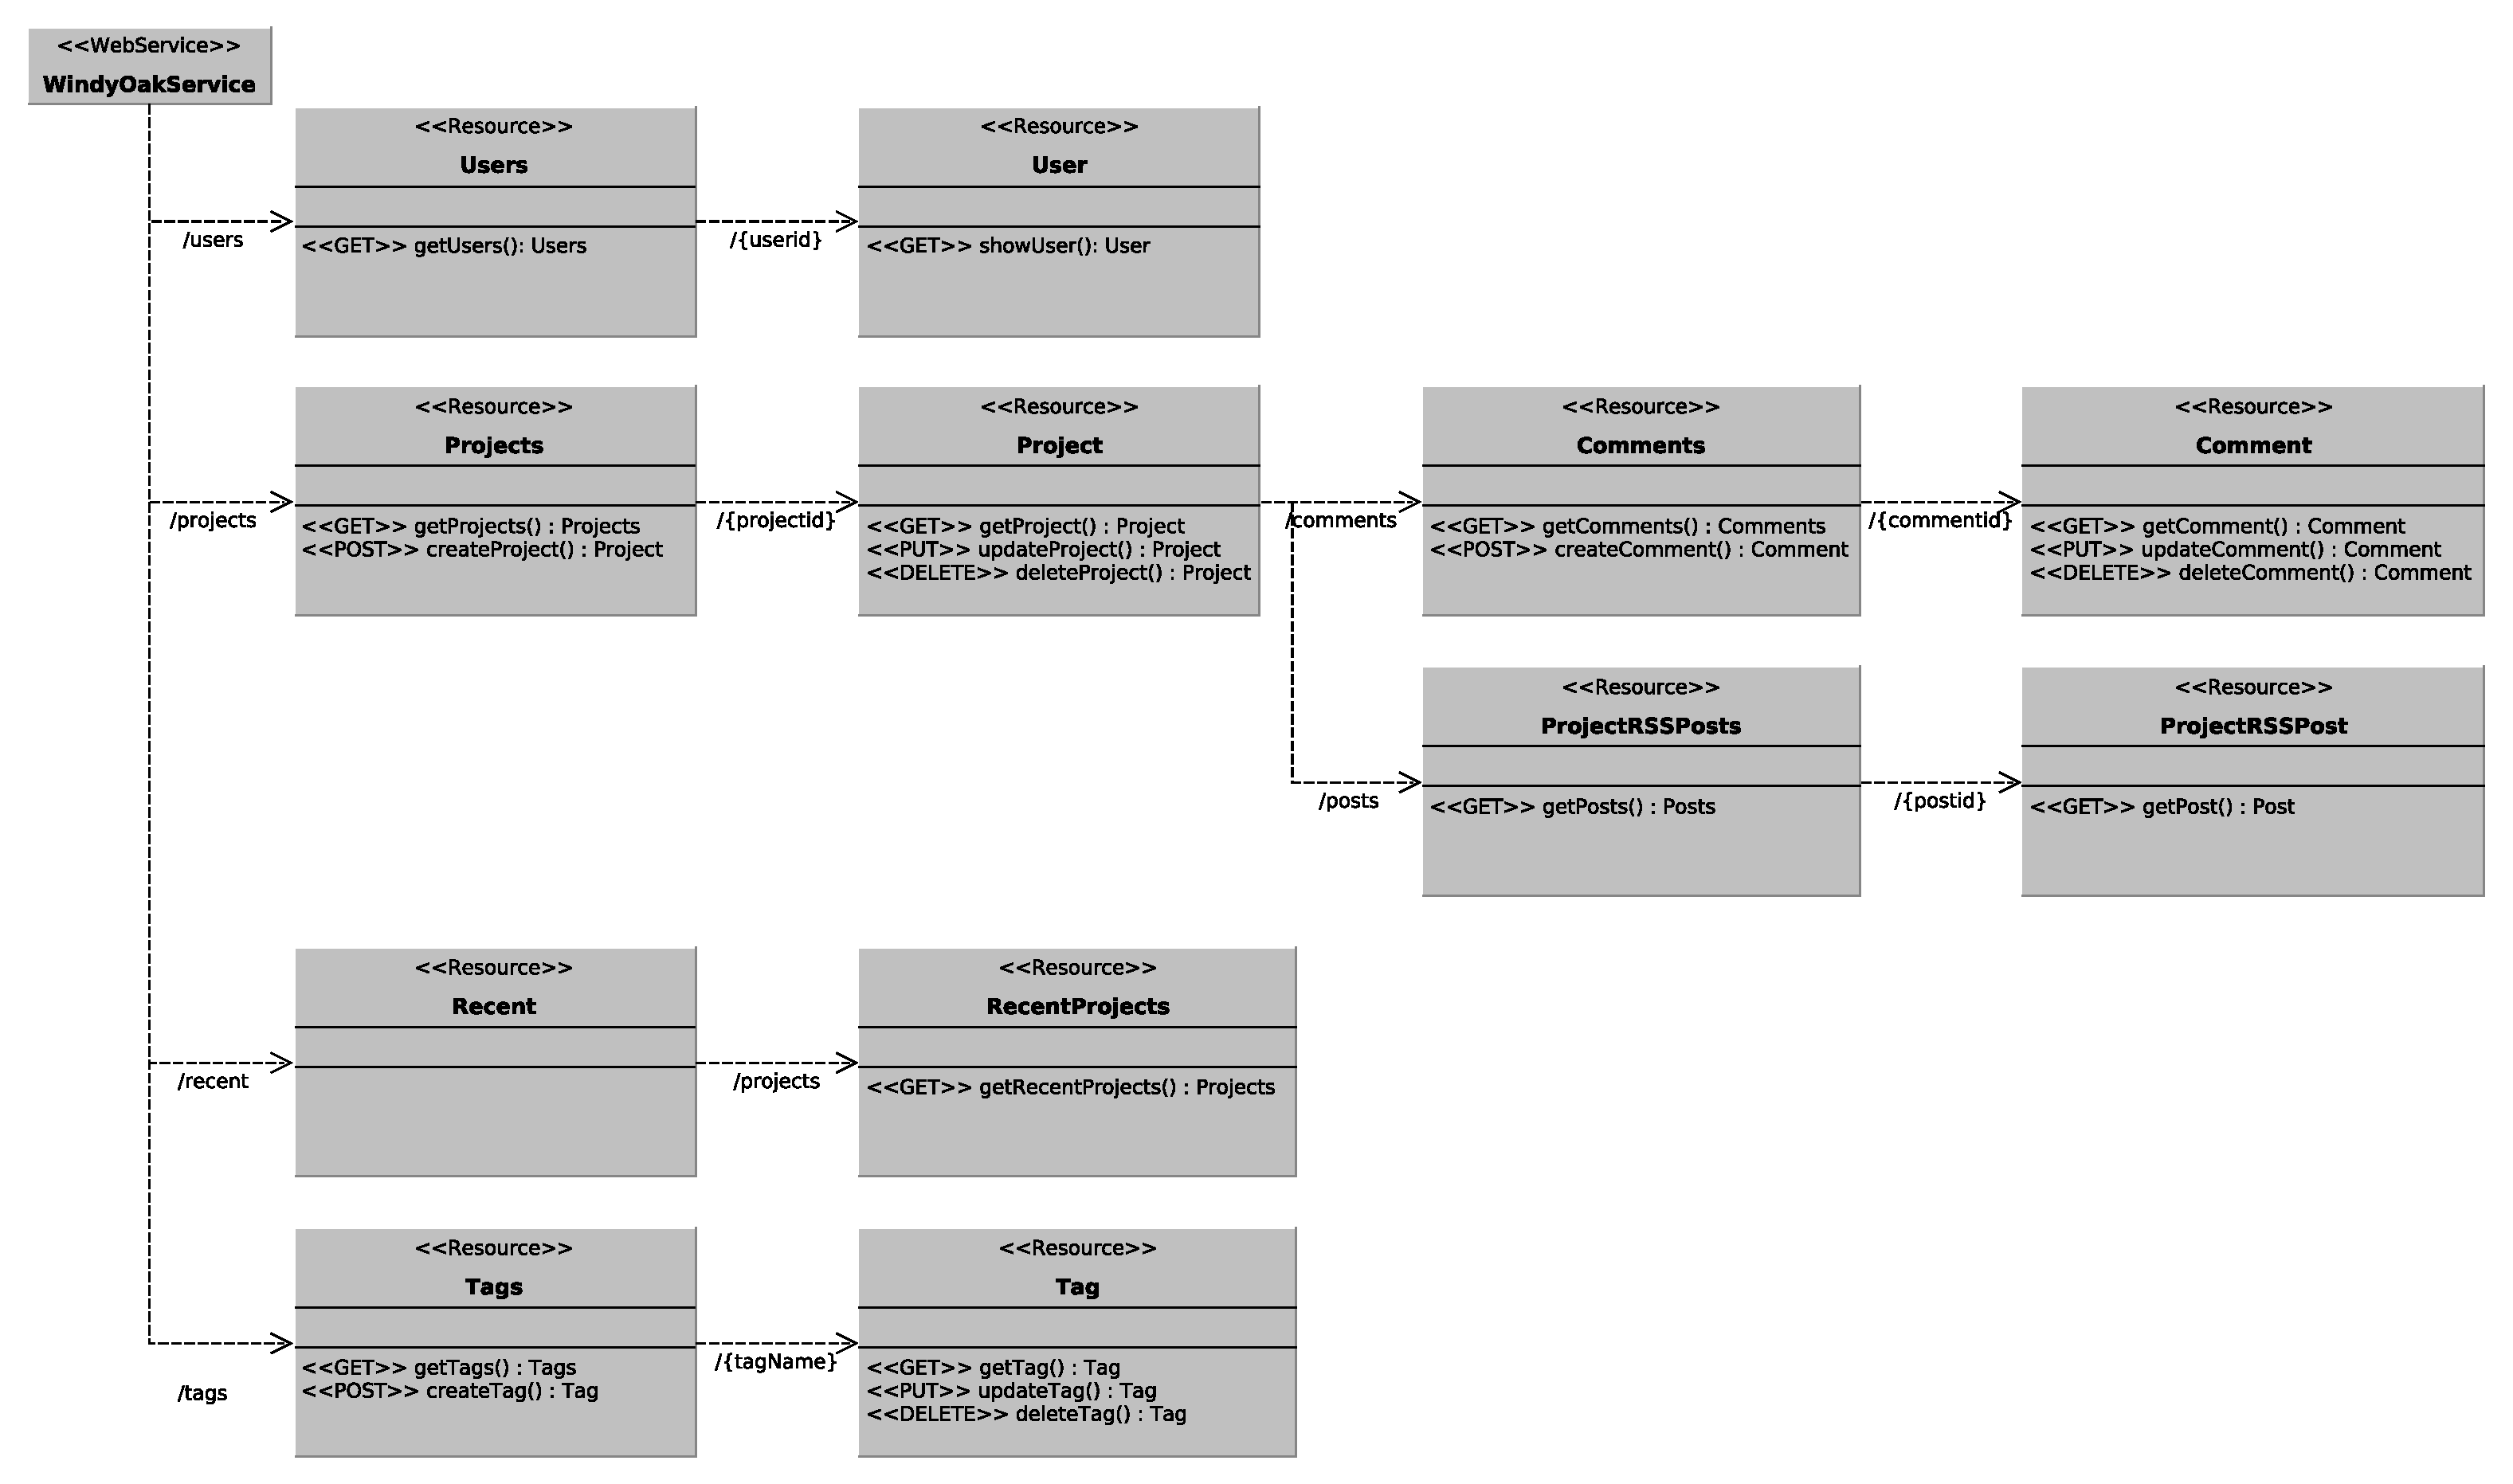
\includegraphics[width=\linewidth,height=\textheight,keepaspectratio]{../Bilder/rest.pdf} 
			  \caption{REST-Schnittstelle im Überblick}
			  \label{fig:rest}
			 \end{figure}
			\end{landscape}
		\begin{landscape}
			\begin{figure}
  				\centering
  				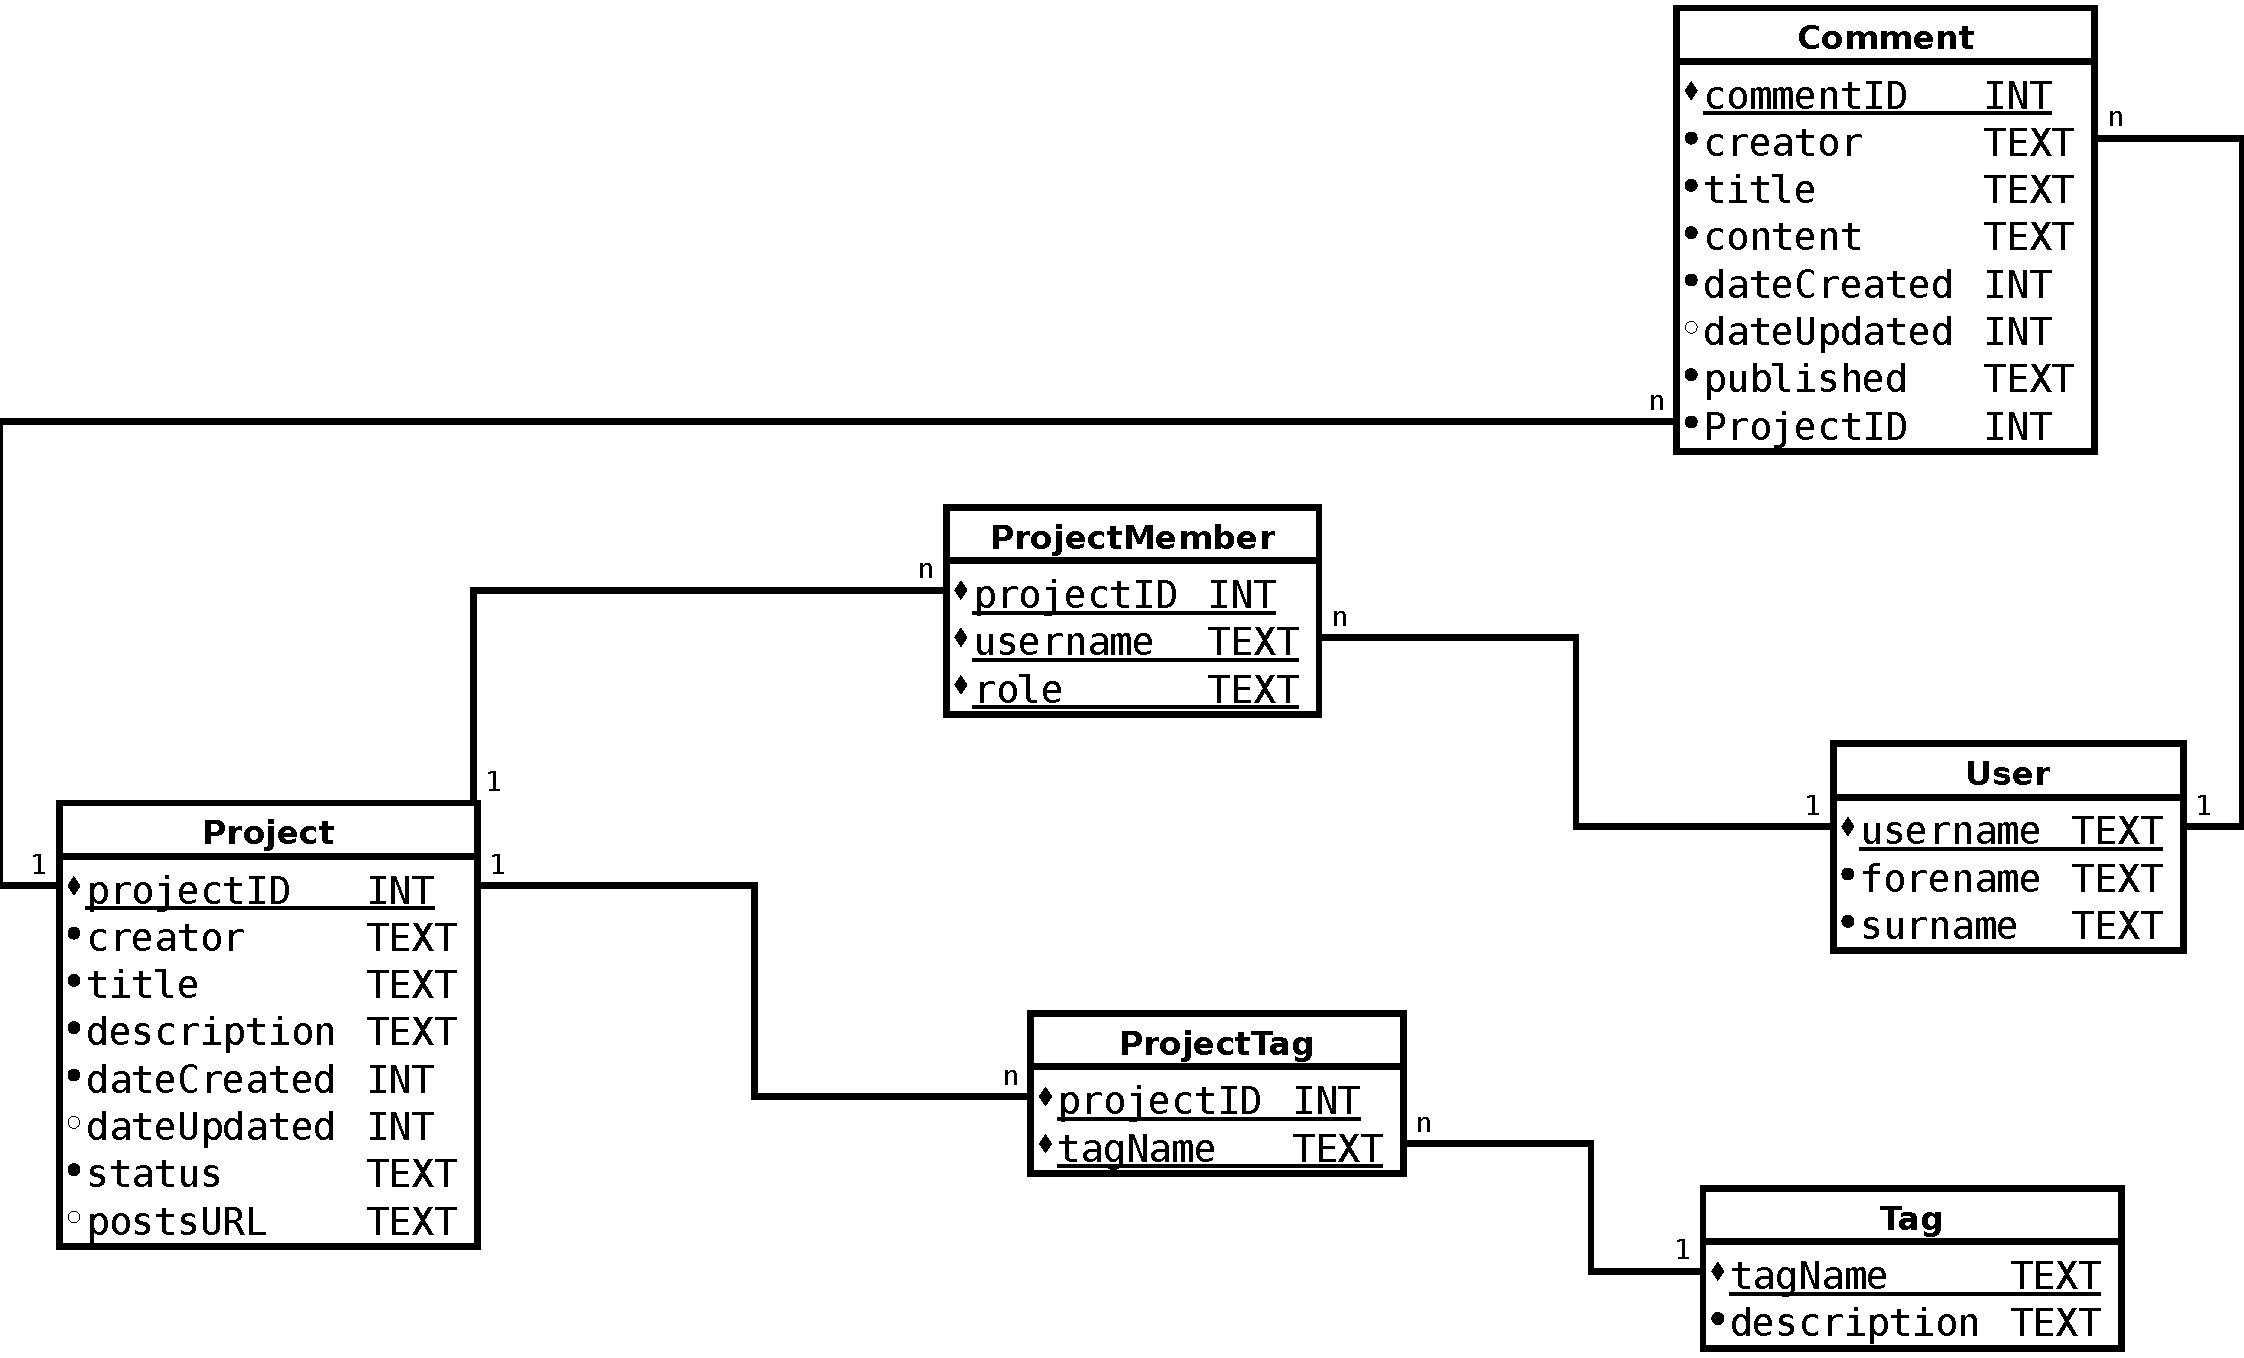
\includegraphics[width=\linewidth,height=\textheight,keepaspectratio]{../Bilder/db.pdf} 
  				\caption{Datenbankschema im Überblick}
  				\label{fig:db}
		 	\end{figure}
		\end{landscape}
		
\end{document}
